The platform is founded on a decoupled architecture designed to promote modularity, scalability, and maintainability. This architectural style separates the system into several distinct, independently deployable components, each with a specific responsibility. This approach prevents the tight coupling of a monolithic system, allowing for greater flexibility in development, technology choice, and scaling strategies. Communication between these modules is handled through a well-defined \acs{api}, which serves as the contract between the frontend client and the backend services.

The primary components of the architecture are:
\begin{compactitem}[\textbullet]
    \item \textbf{Frontend Application:} A client-side \ac{pwa} built with Next.js, which serves as the sole point of interaction for the end-user. It is responsible for rendering the entire user interface and managing client-side state.
    \item \textbf{Backend \acs{api} Gateway:} A central, high-performance \acs{api} developed in FastAPI. This component acts as an orchestrator, handling all business logic, user authentication, and routing requests to the appropriate downstream services.
    \item \textbf{LLM Service:} A dedicated container running Ollama, responsible for hosting, managing, and serving inferences from the open-source \acp{llm}.
    \item \textbf{Data Services:} A collection of data storage solutions, including a Supabase PostgreSQL instance for structured metadata, and a FalkorDB graph database for storing and querying both user-item interaction data and chat history records.
\end{compactitem}

Each of these components is containerized using Docker, ensuring environmental consistency and portability across different deployment stages. This modular design, illustrated in Figure~\ref{FIG:ARCH_OVERVIEW}, is fundamental to achieving the system's non-functional requirements of scalability and maintainability.

\begin{figure}[System Architecture Diagram]{FIG:ARCH_OVERVIEW}{High-Level System Architecture Diagram.}
    \centering
    % 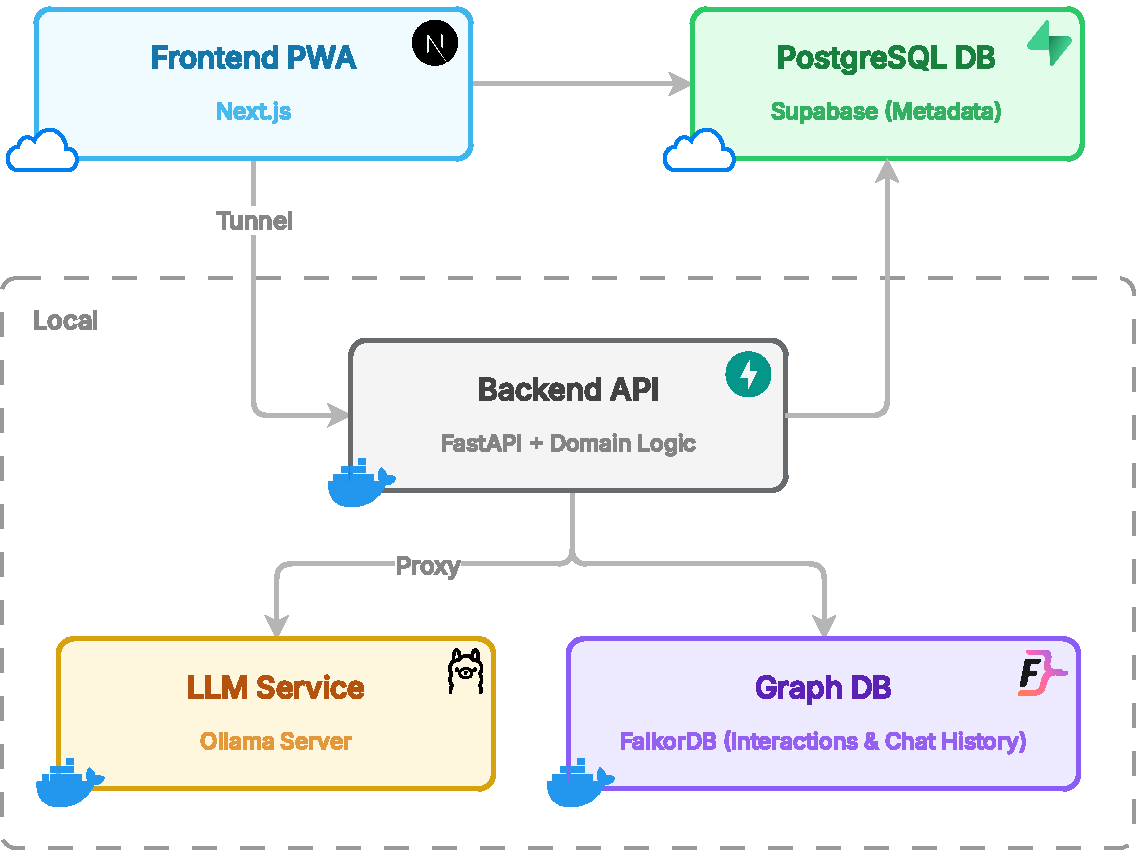
\includegraphics[width=\textwidth]{architecture_overview.png}
    \includesvg[inkscapelatex=false,width=\textwidth]{placeholder}
\end{figure}